\documentclass[a4paper]{article}
\usepackage[utf8]{inputenc}


\title{ Práctica 4 \\
\begin{large}
     Fundamentos de la Ciencia de Datos
\end{large}
}
\author{Samuel Aós Paumard,\\
Enrique Coronado Barco,\\
Carmen Martínez Estévez,\\
Alberto Martínez Ortega}
\usepackage{Sweave}
\begin{document}
\Sconcordance{concordance:practica4.tex:practica4.Rnw:%
1 13 1 1 0 8 1 1 2 1 0 1 1 14 0 1 2 1 1 1 2 1 0 1 1 8 0 1 2 1 1 1 2 23 0 1 2 1 1 1 2 15 0 1 2 1 1 1 2 11 0 1 2 1 1 1 2 11 0 1 2 2 1 1 2 10 0 1 1 10 0 1 2 14 1 1 2 1 0 9 %
1 3 0 1 2 3 1 1 2 1 0 2 1 20 0 1 2 2 1 1 2 1 0 1 1 26 0 1 2 2 1 1 2 1 0 1 1 4 0 1 2 7 1 1 2 1 0 3 1 3 0 1 2 3 1 1 2 1 0 3 1 1 2 4 0 1 2 35 1 1 2 1 0 3 1 14 0 1 2 3 1 1 %
2 100 0 1 2 4 1 1 2 155 0 1 2 6 1 1 2 85 0 1 2 2 1 1 2 1 0 2 1 29 0 1 2 5 1}

\maketitle

\section{Ejericio 1}
\textbf{La primera parte consiste en la realización de un ejercicio en clase con ayuda del profesor en el que se va a realizar un análisis de clasificación no supervisada de Datos con R aplicando todos los conceptos vistos en el tema. En dicho ejercicio se resolverá, utilizando el algoritmo K-means, el mismo problema que el visto en la descripción teórica del tema. Es decir, para la misma muestra1 que se utilizó para hacer de forma manual el primer ejercicio de clasificación no supervisada, se deberán obtener los centroides de los clusters obtenidos.}

Mediante la muestra de calificaciones vista en teoría, compuesta por las calificaciones de Teoría y Laboratorio, realizamos una matriz en cuya transpuesta observamos los valores de la primera columna como los correspondientes a Teoría y la segunda los de Laboratorio.

\begin{Schunk}
\begin{Sinput}
> m<-matrix(c(4,4,3,5,1,2,5,5,0,1,2,2,4,5,2,1),2,8)
> (m<-t(m))
\end{Sinput}
\begin{Soutput}
     [,1] [,2]
[1,]    4    4
[2,]    3    5
[3,]    1    2
[4,]    5    5
[5,]    0    1
[6,]    2    2
[7,]    4    5
[8,]    2    1
\end{Soutput}
\end{Schunk}

Cargamos en la variable \textit{centroides} los valores de los centroides C1=[0,1] y C2=[2,2].
\begin{Schunk}
\begin{Sinput}
> centroides<-matrix(c(0,1,2,2),2,2)
> (centroides<-t(centroides))
\end{Sinput}
\begin{Soutput}
     [,1] [,2]
[1,]    0    1
[2,]    2    2
\end{Soutput}
\end{Schunk}

Realizamos la clasificación k-means usando ambas variables generadas anteriormente.
\begin{Schunk}
\begin{Sinput}
> (clasificacion<-kmeans(m,centroides,4))
\end{Sinput}
\begin{Soutput}
K-means clustering with 2 clusters of sizes 4, 4

Cluster means:
  [,1] [,2]
1 1.25 1.50
2 4.00 4.75

Clustering vector:
[1] 2 2 1 2 1 1 2 1

Within cluster sum of squares by cluster:
[1] 3.75 2.75
 (between_SS / total_SS =  84.8 %)

Available components:

[1] "cluster"      "centers"      "totss"        "withinss"     "tot.withinss" "betweenss"    "size"         "iter"         "ifault"      
\end{Soutput}
\end{Schunk}

Como podemos observar obtenemos un conjunto amplio de valores entre los que cabe destacar los valores de los centroides del cluster obtenido C1=[1.25,1.50] y C2=[4.00,4.75]. Otro valor importante obtenido es el vector cluster, el cual a continuación introduciremos como primera columna de nuestro conjunto de clasificaciones.
\begin{Schunk}
\begin{Sinput}
> (m=cbind(clasificacion$cluster,m))
\end{Sinput}
\begin{Soutput}
     [,1] [,2] [,3]
[1,]    2    4    4
[2,]    2    3    5
[3,]    1    1    2
[4,]    2    5    5
[5,]    1    0    1
[6,]    1    2    2
[7,]    2    4    5
[8,]    1    2    1
\end{Soutput}
\end{Schunk}

Extraemos todos los valores del conjunto de datos los cuales en la primera columna, la indicativa de los valores del cluster, tengan valor 1.
\begin{Schunk}
\begin{Sinput}
> (mc1=subset(m,m[ ,1]==1)) 
\end{Sinput}
\begin{Soutput}
     [,1] [,2] [,3]
[1,]    1    1    2
[2,]    1    0    1
[3,]    1    2    2
[4,]    1    2    1
\end{Soutput}
\end{Schunk}

De igual forma lo hacemos para aquellos valores que correspondan con el cluster de valor 2.
\begin{Schunk}
\begin{Sinput}
> (mc2=subset(m,m[ ,1]==2))
\end{Sinput}
\begin{Soutput}
     [,1] [,2] [,3]
[1,]    2    4    4
[2,]    2    3    5
[3,]    2    5    5
[4,]    2    4    5
\end{Soutput}
\end{Schunk}

Una vez clasificados los datos de acuerdo a sus clusteres, extraemos la columna referente al valor de estos para facilitar la lectura.

\begin{Schunk}
\begin{Sinput}
> (mc1=mc1[,-1])
\end{Sinput}
\begin{Soutput}
     [,1] [,2]
[1,]    1    2
[2,]    0    1
[3,]    2    2
[4,]    2    1
\end{Soutput}
\begin{Sinput}
> (mc2=mc2[,-1])
\end{Sinput}
\begin{Soutput}
     [,1] [,2]
[1,]    4    4
[2,]    3    5
[3,]    5    5
[4,]    4    5
\end{Soutput}
\end{Schunk}

\newpage
\section{Ejericio 2}
\textbf{La segunda parte consiste en el Desarrollo por parte de cada alumno del enunciado y la solución de un ejercicio en el que se realice un análisis con R de clasificación no supervisada introduciendo modificaciones sobre el ejercicio hecho en clase.}

En cuanto a las librerías usadas para esta parte, encontramos:
\begin{itemize}
     \item tidyverse: conjunto de paquetes de R especialmente desarollados para Ciencia de Datos y una mayor correlación entre ellos con sintaxis común, por ejemplo.
     \item cluster: métodos para análisis de clusters de datos. Más extendido que su predecesor de 1990 "Finding Groups in Data".
     \item factoextra: extrae y muestra los datos de manera sencilla. También tiene métodos para simplificar algunos análisis de clusters.
     \item gridExtra: permite agrupar múltiples gráficas en una sola o dibujar tablas.
     \item magick: procesamiento de imagen de una forma sencilla sin perder eficacia. Necesario para LearnClust.
     \item LearnClust: para el ejercicio 3, será explicado convenientemente más adelante.
\end{itemize}

\begin{Schunk}
\begin{Sinput}
> install.packages("LearnClust")
> install.packages("factoextra")
> install.packages("xlsx")
> install.packages("magick")
> library(tidyverse)
> library(cluster)
> library(factoextra)
> library(gridExtra)
> library(magick)
> library(LearnClust)
\end{Sinput}
\end{Schunk}

En este caso, la muestra utilizada es otra de calificaciones modificada a partir de la anterior. Encontramos cinco columnas esta vez, frente a las dos anteriores. Esto es porque además de las notas de teoría y laboratorio se han añadido las calificaciones medias de prácticas, ensayos y entregas.
Si los cargamos desde el .txt donde están y eliminamos los valores NA, en caso de haberlos, obtenemos la siguiente matriz de datos:

\begin{Schunk}
\begin{Sinput}
> calificaciones<-read.table("calificaciones.txt")
> calificaciones<-na.omit(calificaciones)
> calificaciones
\end{Sinput}
\begin{Soutput}
        Teoria Laboratorio Practicas Ensayo Entregas
Javier     7.4         6.3       5.5    7.6      3.2
Jorge      5.2         4.9       4.4    6.0      6.5
Ivan       7.3         8.5       9.6    6.7      5.8
Ruben      7.2         6.0       6.0    6.0      7.0
Ana        5.0         5.0       5.0    6.5      5.0
Sara       7.0         7.0       7.0    8.6      7.0
Sonia      0.0         1.0       2.0    5.4      5.0
Alvaro     8.0         7.0       4.0    5.0      6.0
Carmen     7.0         6.0       7.0    8.0      8.0
Jaime      0.0         1.0       2.0    0.0      0.0
Elisa     10.0        10.0      10.0    9.0     10.0
Arturo     8.0         9.0       8.0    2.0      8.0
Beltran    7.0         8.0       9.0    9.0      9.0
Samuel     8.0         7.0       8.0    9.0      9.0
\end{Soutput}
\end{Schunk}

Como no queremos que el algoritmo de agrupamiento dependa solo de una variable, estandarizamos los datos con scale, obteniendo la siguiente matriz de datos:

\begin{Schunk}
\begin{Sinput}
> calificaciones<-scale(calificaciones)
> calificaciones
\end{Sinput}
\begin{Soutput}
            Teoria Laboratorio   Practicas      Ensayo    Entregas
Javier   0.4069373  0.04071393 -0.29009186  0.47058979 -1.22739862
Jorge   -0.3526790 -0.49128139 -0.71555993 -0.12834267  0.04118787
Ivan     0.3724093  0.87670657  1.29574365  0.13369028 -0.22790623
Ruben    0.3378813 -0.07328507 -0.09669729 -0.12834267  0.23339795
Ana     -0.4217351 -0.45328172 -0.48348644  0.05882372 -0.53544235
Sara     0.2688253  0.30671159  0.29009186  0.84492257  0.23339795
Sonia   -2.1481359 -1.97326835 -1.64385389 -0.35294234 -0.53544235
Alvaro   0.6141055  0.30671159 -0.87027559 -0.50267546 -0.15102220
Carmen   0.2688253 -0.07328507  0.29009186  0.62032290  0.61781810
Jaime   -2.1481359 -1.97326835 -1.64385389 -2.37433939 -2.45754310
Elisa    1.3046658  1.44670155  1.45045931  0.99465569  1.38665840
Arturo   0.6141055  1.06670490  0.67688101 -1.62567381  0.61781810
Beltran  0.2688253  0.68670824  1.06367016  0.99465569  1.00223825
Samuel   0.6141055  0.30671159  0.67688101  0.99465569  1.00223825
attr(,"scaled:center")
     Teoria Laboratorio   Practicas      Ensayo    Entregas 
   6.221429    6.192857    6.250000    6.342857    6.392857 
attr(,"scaled:scale")
     Teoria Laboratorio   Practicas      Ensayo    Entregas 
   2.896199    2.631602    2.585388    2.671420    2.601320 
\end{Soutput}
\end{Schunk}

A continuación calculamos una matriz de distancia entre las filas, que será usada posteriormente para la visualización de esta según colores, dependiendo de si la distancia es 'baja', 'media' o 'alta'.

\begin{Schunk}
\begin{Sinput}
> distancia<-get_dist(calificaciones)
> fviz_dist(distancia, gradient = list(low = "#FDFEFF", mid = "#84B5E6", high = "#020D6C"))
\end{Sinput}
\end{Schunk}
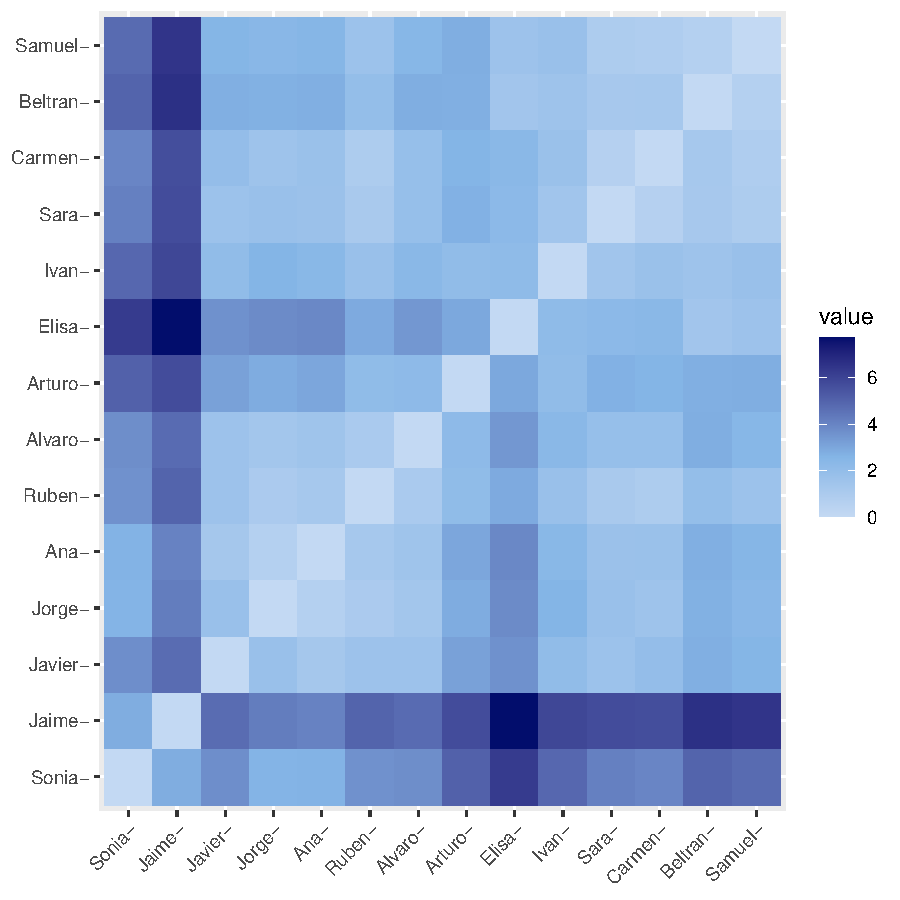
\includegraphics{practica4-011}

Estudiamos los distintos casos con el algoritmo kmeans. Como parámetros a esta función encontramos los siguientes. 
\begin{itemize}
     \item calificaciones: matriz estandarizada con los datos a estudiar.
     \item centers={1,2,3,4}: al ser un número, significa el número de filas (distintas) que se van a escoger como centroides iniciales.
     \item nstart: si centers es un número, que lo es, hace referencia a cuántos sets aleatorios han de ser escogidos para llevar a cabo el método.
\end{itemize}

\begin{Schunk}
\begin{Sinput}
> k2 <- kmeans(calificaciones, centers = 1, nstart = 25)
> k3 <- kmeans(calificaciones, centers = 2, nstart = 25)
> k4 <- kmeans(calificaciones, centers = 3, nstart = 25)
> k5 <- kmeans(calificaciones, centers = 4, nstart = 25)
\end{Sinput}
\end{Schunk}

Una vez obtenidos los resultados de los 4 kmeans realizados, procedemos a mostrarlos en una gráfica a la que le pasamos la variable que guarda los resultados de cada uno, las calificaciones sobre las que se han obtenido dichos resultados y agregamos un título a cada una para tenerlas identificadas.
Esto es así porque, para mostrar los datos de una manera más ordenada y cuya comparación resulte más fácil, se han agrupado las 4 gráficas en una sola.

\begin{Schunk}
\begin{Sinput}
> p1<-fviz_cluster(k2, data = calificaciones) + ggtitle("K = 1")
> p2<-fviz_cluster(k3, data = calificaciones) + ggtitle("K = 2")
> p3<-fviz_cluster(k4, data = calificaciones) + ggtitle("K = 3")
> p4<-fviz_cluster(k5, data = calificaciones) + ggtitle("K = 4")
> grid.arrange(p1, p2, p3,p4, nrow = 2)
\end{Sinput}
\end{Schunk}
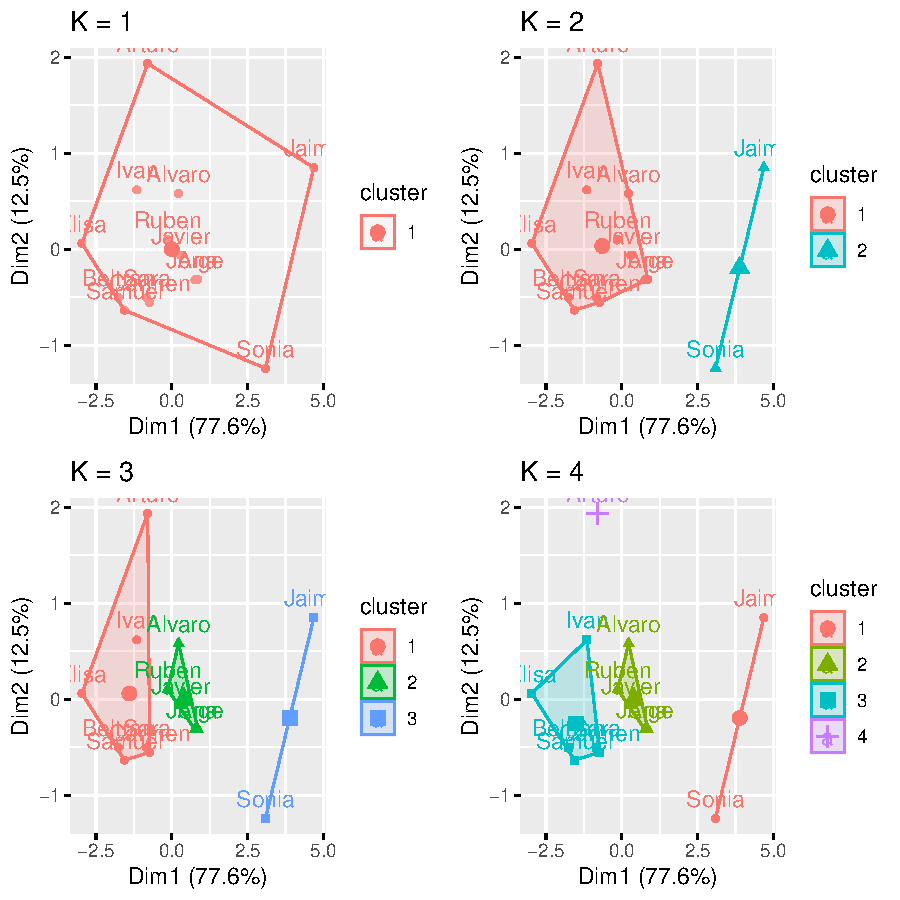
\includegraphics{practica4-graficas2}
\\

Si observamos los resultados obtenemos las siguientes conclusiones:
Con k=1, es decir, un único centroide, todos los datos están agrupados bajo la misma clase, incluso los más alejados del centro, pues no hay más puntos de referencia.
Con k=2, es decir, dos centroides, vemos como Sonia y Jaime, que eran los más alejados ya pertenecen a otra clase distinta que el resto de los datos, que siguen pertenenciendo al primer centroide.
Con k=3, ocurre una cosa curiosa y es que Sonia y Jaime están tan alejados del resto de los datos y entre sí, que la clasificación hace que se separen en 2 clases distintas, dejando el resto de los datos sin modificar.
Con k=4, Sonia y Jaime siguen estando como antes. La diferencia se aprecia en los datos que pertenecían a la clase 'roja', que ha quedado dividida en dos clases diferentes, ajustando los centroides.

\newpage
\section{Ejericio 3}
\textbf{Aplicar y analizar el paquete de R: LearnClust: Learning Hierarchical Clustering Algorithms}

Se trata de un paquete realizado por un alumno de la UAH donde se nos permite conocer a fondo los entresijos de la clusterización jerárquica, aglomerativa y divisiva.
Cada función ofrece una opción ".details" que nos detalla, paso a paso, cómo se va iterando y calculando el resultado final. Además, permite el uso de funciones distancia, inicialización de datos y otras funciones de interés que favorecen un estudio profundo de estos algoritmos, su recodificación con posibles mejoras, así como una realización del propio algoritmo de manera más detallada y parcial, según interese al usuario.
El paquete contiene 3 funciones para realizar clustering, cada una con su .details. Hemos realizado un análisis de los resultados con cada uno de los 3 tipos: aglomerativeHC, divisiveHC, correlationHC.
Las 2 primeras funciones aceptan los 3 mismos parámetros:
\begin{itemize}
     \item data: matriz, vector o dataframe numérico. Será transformado a matriz y lista
     \item distance: tipo de distancia usado. Existen diversos tipos:
      \begin{itemize}
          \item CAN: Distancia Canberra
          \item CHE: Distancia Chebyshev
          \item EUC: Distancia Euclídea 
          \item MAN: Distancia Manhattan 
          \item OCT: Distancia Octil
      \end{itemize}
     \item approach: una vez calculada la distancia, tipo de acercamiento usado. Existen diversos tipos:
      \begin{itemize}
          \item MAX: Máximo del vector
          \item MIN: Mínimo del vector
          \item AVG: Media del vector
      \end{itemize}
\end{itemize}

Definimos la matriz a utilizar y la convertimos a dataframe.

\begin{Schunk}
\begin{Sinput}
> matrizA<-c(4,4,3,5,1,2,5,5,0,1,2,2,4,5,2,1)
> matriz<-matrix(matrizA,ncol=2)
> matriz<-data.frame(matriz)
> matriz
\end{Sinput}
\begin{Soutput}
  X1 X2
1  4  0
2  4  1
3  3  2
4  5  2
5  1  4
6  2  5
7  5  2
8  5  1
\end{Soutput}
\end{Schunk}

Comenzamos con el aglomerativeHC, distancia: euclídea, aproach: máximo.
Según la documentación del método, los datos son formateados y se crean los clusters, calculando la matriz de distancias con los parámetros seleccionados. Se escoge la distancia y los clusters. Estos se agrupan en uno nuevo y actualiza la lista de clusters. Se itera hasta que solo existe un único cluster.
Los resultados son los siguientes:
\begin{Schunk}
\begin{Sinput}
> agglomerativeHC(matriz, 'EUC', 'MAX')
\end{Sinput}
\begin{Soutput}
$dendrogram
Number of objects: 8 


$clusters
$clusters[[1]]
  X1 X2
1  4  0

$clusters[[2]]
  X1 X2
1  4  1

$clusters[[3]]
  X1 X2
1  3  2

$clusters[[4]]
  X1 X2
1  5  2

$clusters[[5]]
  X1 X2
1  1  4

$clusters[[6]]
  X1 X2
1  2  5

$clusters[[7]]
  X1 X2
1  5  2

$clusters[[8]]
  X1 X2
1  5  1

$clusters[[9]]
  X1 X2
1  4  0
2  4  1

$clusters[[10]]
  X1 X2
1  5  2
2  5  1

$clusters[[11]]
  X1 X2
1  5  2
2  5  2
3  5  1

$clusters[[12]]
  X1 X2
1  1  4
2  2  5

$clusters[[13]]
  X1 X2
1  3  2
2  4  0
3  4  1

$clusters[[14]]
  X1 X2
1  5  2
2  5  2
3  5  1
4  3  2
5  4  0
6  4  1

$clusters[[15]]
  X1 X2
1  1  4
2  2  5
3  5  2
4  5  2
5  5  1
6  3  2
7  4  0
8  4  1


$groupedClusters
  cluster1 cluster2
1        1        2
2        4        8
3        7       10
4        5        6
5        3        9
6       11       13
7       12       14
\end{Soutput}
\end{Schunk}

\newpage

Si ejecutamos la version .details podemos observar una cantidad abrumadora de explicaciones sobre todos los cálculos realizados a lo largo de la ejecución del algoritmo. Por supuesto, al final se nos muestra el resultado, que es idéntico al obtenido anteriormente.

\begin{Schunk}
\begin{Sinput}
> agglomerativeHC.details(matriz, 'EUC', 'MAX')
\end{Sinput}
\begin{Soutput}
[[1]]
     [,1] [,2] [,3]
[1,]    4    0    1

[[2]]
     [,1] [,2] [,3]
[1,]    4    1    1

[[3]]
     [,1] [,2] [,3]
[1,]    3    2    1

[[4]]
     [,1] [,2] [,3]
[1,]    5    2    1

[[5]]
     [,1] [,2] [,3]
[1,]    1    4    1

[[6]]
     [,1] [,2] [,3]
[1,]    2    5    1

[[7]]
     [,1] [,2] [,3]
[1,]    5    2    1

[[8]]
     [,1] [,2] [,3]
[1,]    5    1    1

         [,1]     [,2]     [,3]     [,4]     [,5]     [,6]     [,7]     [,8]
[1,] 0.000000 1.000000 2.236068 2.236068 5.000000 5.385165 2.236068 1.414214
[2,] 1.000000 0.000000 1.414214 1.414214 4.242641 4.472136 1.414214 1.000000
[3,] 2.236068 1.414214 0.000000 2.000000 2.828427 3.162278 2.000000 2.236068
[4,] 2.236068 1.414214 2.000000 0.000000 4.472136 4.242641 0.000000 1.000000
[5,] 5.000000 4.242641 2.828427 4.472136 0.000000 1.414214 4.472136 5.000000
[6,] 5.385165 4.472136 3.162278 4.242641 1.414214 0.000000 4.242641 5.000000
[7,] 2.236068 1.414214 2.000000 0.000000 4.472136 4.242641 0.000000 1.000000
[8,] 1.414214 1.000000 2.236068 1.000000 5.000000 5.000000 1.000000 0.000000
  X1 X2
1  4  0
2  4  1
      [,1] [,2]     [,3]     [,4]     [,5]     [,6]     [,7]     [,8]     [,9]
 [1,]    0    0 0.000000 0.000000 0.000000 0.000000 0.000000 0.000000 0.000000
 [2,]    0    0 0.000000 0.000000 0.000000 0.000000 0.000000 0.000000 0.000000
 [3,]    0    0 0.000000 2.000000 2.828427 3.162278 2.000000 2.236068 2.236068
 [4,]    0    0 2.000000 0.000000 4.472136 4.242641 0.000000 1.000000 2.236068
 [5,]    0    0 2.828427 4.472136 0.000000 1.414214 4.472136 5.000000 5.000000
 [6,]    0    0 3.162278 4.242641 1.414214 0.000000 4.242641 5.000000 5.385165
 [7,]    0    0 2.000000 0.000000 4.472136 4.242641 0.000000 1.000000 2.236068
 [8,]    0    0 2.236068 1.000000 5.000000 5.000000 1.000000 0.000000 1.414214
 [9,]    0    0 2.236068 2.236068 5.000000 5.385165 2.236068 1.414214 0.000000
  X1 X2
1  5  2
2  5  1
      [,1] [,2]     [,3] [,4]     [,5]     [,6]     [,7] [,8]     [,9]    [,10]
 [1,]    0    0 0.000000    0 0.000000 0.000000 0.000000    0 0.000000 0.000000
 [2,]    0    0 0.000000    0 0.000000 0.000000 0.000000    0 0.000000 0.000000
 [3,]    0    0 0.000000    0 2.828427 3.162278 2.000000    0 2.236068 2.236068
 [4,]    0    0 0.000000    0 0.000000 0.000000 0.000000    0 0.000000 0.000000
 [5,]    0    0 2.828427    0 0.000000 1.414214 4.472136    0 5.000000 5.000000
 [6,]    0    0 3.162278    0 1.414214 0.000000 4.242641    0 5.385165 5.000000
 [7,]    0    0 2.000000    0 4.472136 4.242641 0.000000    0 2.236068 1.000000
 [8,]    0    0 0.000000    0 0.000000 0.000000 0.000000    0 0.000000 0.000000
 [9,]    0    0 2.236068    0 5.000000 5.385165 2.236068    0 0.000000 2.236068
[10,]    0    0 2.236068    0 5.000000 5.000000 1.000000    0 2.236068 0.000000
  X1 X2
1  5  2
2  5  2
3  5  1
      [,1] [,2]     [,3] [,4]     [,5]     [,6] [,7] [,8]     [,9] [,10]    [,11]
 [1,]    0    0 0.000000    0 0.000000 0.000000    0    0 0.000000     0 0.000000
 [2,]    0    0 0.000000    0 0.000000 0.000000    0    0 0.000000     0 0.000000
 [3,]    0    0 0.000000    0 2.828427 3.162278    0    0 2.236068     0 2.236068
 [4,]    0    0 0.000000    0 0.000000 0.000000    0    0 0.000000     0 0.000000
 [5,]    0    0 2.828427    0 0.000000 1.414214    0    0 5.000000     0 5.000000
 [6,]    0    0 3.162278    0 1.414214 0.000000    0    0 5.385165     0 5.000000
 [7,]    0    0 0.000000    0 0.000000 0.000000    0    0 0.000000     0 0.000000
 [8,]    0    0 0.000000    0 0.000000 0.000000    0    0 0.000000     0 0.000000
 [9,]    0    0 2.236068    0 5.000000 5.385165    0    0 0.000000     0 2.236068
[10,]    0    0 0.000000    0 0.000000 0.000000    0    0 0.000000     0 0.000000
[11,]    0    0 2.236068    0 5.000000 5.000000    0    0 2.236068     0 0.000000
  X1 X2
1  1  4
2  2  5
      [,1] [,2]     [,3] [,4] [,5] [,6] [,7] [,8]     [,9] [,10]    [,11]    [,12]
 [1,]    0    0 0.000000    0    0    0    0    0 0.000000     0 0.000000 0.000000
 [2,]    0    0 0.000000    0    0    0    0    0 0.000000     0 0.000000 0.000000
 [3,]    0    0 0.000000    0    0    0    0    0 2.236068     0 2.236068 3.162278
 [4,]    0    0 0.000000    0    0    0    0    0 0.000000     0 0.000000 0.000000
 [5,]    0    0 0.000000    0    0    0    0    0 0.000000     0 0.000000 0.000000
 [6,]    0    0 0.000000    0    0    0    0    0 0.000000     0 0.000000 0.000000
 [7,]    0    0 0.000000    0    0    0    0    0 0.000000     0 0.000000 0.000000
 [8,]    0    0 0.000000    0    0    0    0    0 0.000000     0 0.000000 0.000000
 [9,]    0    0 2.236068    0    0    0    0    0 0.000000     0 2.236068 5.385165
[10,]    0    0 0.000000    0    0    0    0    0 0.000000     0 0.000000 0.000000
[11,]    0    0 2.236068    0    0    0    0    0 2.236068     0 0.000000 5.000000
[12,]    0    0 3.162278    0    0    0    0    0 5.385165     0 5.000000 0.000000
  X1 X2
1  3  2
2  4  0
3  4  1
      [,1] [,2] [,3] [,4] [,5] [,6] [,7] [,8] [,9] [,10]    [,11]    [,12]    [,13]
 [1,]    0    0    0    0    0    0    0    0    0     0 0.000000 0.000000 0.000000
 [2,]    0    0    0    0    0    0    0    0    0     0 0.000000 0.000000 0.000000
 [3,]    0    0    0    0    0    0    0    0    0     0 0.000000 0.000000 0.000000
 [4,]    0    0    0    0    0    0    0    0    0     0 0.000000 0.000000 0.000000
 [5,]    0    0    0    0    0    0    0    0    0     0 0.000000 0.000000 0.000000
 [6,]    0    0    0    0    0    0    0    0    0     0 0.000000 0.000000 0.000000
 [7,]    0    0    0    0    0    0    0    0    0     0 0.000000 0.000000 0.000000
 [8,]    0    0    0    0    0    0    0    0    0     0 0.000000 0.000000 0.000000
 [9,]    0    0    0    0    0    0    0    0    0     0 0.000000 0.000000 0.000000
[10,]    0    0    0    0    0    0    0    0    0     0 0.000000 0.000000 0.000000
[11,]    0    0    0    0    0    0    0    0    0     0 0.000000 5.000000 2.236068
[12,]    0    0    0    0    0    0    0    0    0     0 5.000000 0.000000 5.385165
[13,]    0    0    0    0    0    0    0    0    0     0 2.236068 5.385165 0.000000
  X1 X2
1  5  2
2  5  2
3  5  1
4  3  2
5  4  0
6  4  1
      [,1] [,2] [,3] [,4] [,5] [,6] [,7] [,8] [,9] [,10] [,11]    [,12] [,13]    [,14]
 [1,]    0    0    0    0    0    0    0    0    0     0     0 0.000000     0 0.000000
 [2,]    0    0    0    0    0    0    0    0    0     0     0 0.000000     0 0.000000
 [3,]    0    0    0    0    0    0    0    0    0     0     0 0.000000     0 0.000000
 [4,]    0    0    0    0    0    0    0    0    0     0     0 0.000000     0 0.000000
 [5,]    0    0    0    0    0    0    0    0    0     0     0 0.000000     0 0.000000
 [6,]    0    0    0    0    0    0    0    0    0     0     0 0.000000     0 0.000000
 [7,]    0    0    0    0    0    0    0    0    0     0     0 0.000000     0 0.000000
 [8,]    0    0    0    0    0    0    0    0    0     0     0 0.000000     0 0.000000
 [9,]    0    0    0    0    0    0    0    0    0     0     0 0.000000     0 0.000000
[10,]    0    0    0    0    0    0    0    0    0     0     0 0.000000     0 0.000000
[11,]    0    0    0    0    0    0    0    0    0     0     0 0.000000     0 0.000000
[12,]    0    0    0    0    0    0    0    0    0     0     0 0.000000     0 5.385165
[13,]    0    0    0    0    0    0    0    0    0     0     0 0.000000     0 0.000000
[14,]    0    0    0    0    0    0    0    0    0     0     0 5.385165     0 0.000000
  X1 X2
1  1  4
2  2  5
3  5  2
4  5  2
5  5  1
6  3  2
7  4  0
8  4  1
\end{Soutput}
\end{Schunk}

Al correr el comando 'Sweave("practica4.Rnw")', se nos ofrece una descripción detallada de los pasos del algoritmo que no hemos conseguido traspasar al .tex para mostrarlo en el pdf.
Como correr otra vez las versiones .details nos dejaría un pdf demasiado largo, hemos omitido esta comprobación en el resto.

Vamos ahora con el divisiveHC, distancia: chebyshev, approach: mínimo.
Volviendo a referirnos al manual, el algoritmo trata lo siguiente: primero se formatean los datos y se crea un cluster que incluye cada uno de los elementos. Posteriormente inicializa otros clusters usando los elementos iniciales. Se calcula una matriz de distancias con los clusters creados en el tercer paso y se escoge la distancia maxima para dividir los clusters. Se dividen en dos clusters complementarios cada uno y se actualiza la lista de clusters. Esto se hace en repetidas ocasiones hasta que cada cluster no pueda ser dividido otra vez. El resultado final es una lista con todos los clusters simples. Los resultados obtenidos son los siguientes:

\begin{Schunk}
\begin{Sinput}
> divisiveHC(matrizA,'CHE','MIN')
\end{Sinput}
\begin{Soutput}
[[1]]
  X1 X2
1  4  4
2  3  5
3  1  2
4  5  5
5  0  1
6  2  2
7  4  5
8  2  1

[[2]]
  X1 X2
1  1  2
2  0  1
3  2  2
4  2  1

[[3]]
  X1 X2
1  4  4
2  3  5
3  5  5
4  4  5

[[4]]
  X1 X2
1  0  1

[[5]]
  X1 X2
1  1  2
2  2  2
3  2  1

[[6]]
  X1 X2
1  4  4

[[7]]
  X1 X2
1  3  5
2  5  5
3  4  5

[[8]]
  X1 X2
1  1  2

[[9]]
  X1 X2
1  2  2
2  2  1

[[10]]
  X1 X2
1  3  5

[[11]]
  X1 X2
1  5  5
2  4  5

[[12]]
  X1 X2
1  2  1

[[13]]
  X1 X2
1  2  2

[[14]]
  X1 X2
1  4  5

[[15]]
  X1 X2
1  5  5
\end{Soutput}
\end{Schunk}
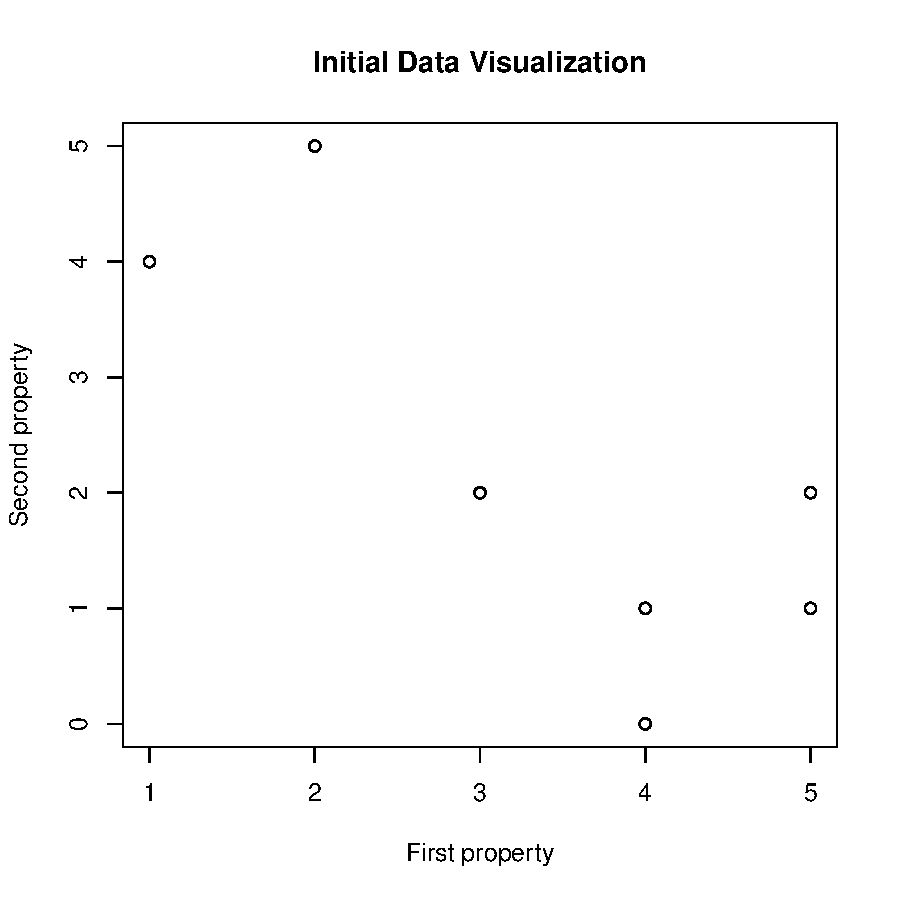
\includegraphics{practica4-divisivo}

Por último, vamos a hacer referencia la método correlationHC. Se diferencia de los dos anteriores en que admite una serie de parámetros más larga que los anteriores. Si bien comparte los anteriores, añade otros como un target(NULL por defecto), unos pesos a considerar en cada paso, si queremos o no normalizar los pesos y una opción para obtener una salida gráfica.
Obtenemos los siguientes resultados para el target y el peso escogidos.
\begin{Schunk}
\begin{Sinput}
> target<- c(2,3)
> weight<- c(1,5)
> correlationHC(matriz,target,weight)
\end{Sinput}
\begin{Soutput}
$sortedValues
  cluster X1 X2
1       3  3  2
2       5  1  4
3       4  5  2
4       7  5  2
5       6  2  5
6       2  4  1
7       8  5  1
8       1  4  0

$distances
  cluster sortedDistances
1       3        1.000000
2       5        1.000000
3       4        1.527525
4       7        1.527525
5       6        1.825742
6       2        2.000000
7       8        2.198484
8       1        2.857738

$dendrogram
Number of objects: 8 
\end{Soutput}
\end{Schunk}

Para terminar, nos gustaría dejar claro que consideramos al LearnClust un paquete muy completo. Permite un aprendizaje en profundidad sobre clustering, quizá en algunos momentos con algo de sobreinformación, pero mejor eso que no tener ni idea de lo que sucede en los entresijos de los algoritmos.
Nos gusta especialmente porque permite hacer cálculos sueltos sobre distancias, incluyendo muchos tipos para calcularlas. También destacamos el hecho de que existan multitud de métodos para poder modificar de manera exahustiva el comportamiento de los algoritmos, así como el poder recodificarlos, modificarlos, ampliarlos o incluso reducirlos a conveniencia. 
Permite una libertad total para la experimentación con este tipo de problemas. De hecho, se podría usar para realizar cáclulos complejos, tediosos a mano, que no tuvieran nada que ver con el clustering. Sirve también para el desarrollo de problemas de clase si queremos comparar algún resultado completo o parte de un procedimiento y no tener que hacerlo todo entero de manera opaca.

\end{document}
